[134 r\textsuperscript{o}] pour les placques ces deux efforts ne seroient pas unis ensemble. Mais il y auroit une difference tres considerable pour la liqueur\protect\index{Sachverzeichnis}{liqueur!purg\'{e}e} purg\'{e}e. Car si on essaye le Mercure purg\'{e}\protect\index{Sachverzeichnis}{mercure!purg\'{e}} dans l'air libre, il sera seulement pouss\'{e} en haut par la pression de l'atmosphere\protect\index{Sachverzeichnis}{atmosph\`{e}re}, \edtext{mais la force unitive du}{\lemma{mais}\Afootnote{ \textit{ (1) }\ l'effort du \textit{ (2) }\  la force unitive du \textit{ L}}} mouuement general\edtext{}{\lemma{}\Afootnote{general  \textbar\ ne \textit{ gestr.}\ \textbar\ le \textit{ L}}} le poussera vers la superficie interieure du verre en tous sens. C'est \`{a} dire aussi bien vers le haut, ou vers le fonds du tuyau renvers\'{e}, que vers les costez du verre: de sorte que seulement l'effort de la force unitive qui va en haut estant detruit par la concurrence de la pression de l'air\protect\index{Sachverzeichnis}{pression de l'air} en même ligne; (selon cette hypothese) toutes les autres pressions de la force unitive resteront, et estant jointes \`{a} celle de l'atmosphere\protect\index{Sachverzeichnis}{atmosph\`{e}re} soûtiendront la liqueur purg\'{e}e\protect\index{Sachverzeichnis}{liqueur!purg\'{e}e}, outre la hauteur ordinaire. C'est donc \`{a} l'experience de determiner si la liqueur\protect\index{Sachverzeichnis}{liqueur!purg\'{e}e} \edtext{purg\'{e}e est attach\'{e}e}{\lemma{liqueur}\Afootnote{ \textit{ (1) }\ s'attache dans le vuide\protect\index{Sachverzeichnis}{vide|textit} \textit{ (2) }\  purg\'{e}e est attach\'{e}e \textit{ L}}} en quelque fa\c{c}on aux costez du tuyau, et si la force qui soûtient les placques dans l'air libre, est plus grande que celle de l'atmosphere\protect\index{Sachverzeichnis}{atmosph\`{e}re}. Car on en pourra juger par l\`{a} de la penetrabilit\'{e} %  @@@ G R A F I K @@@% \begin{wrapfigure}{l}{0.4\textwidth}                    
                %\includegraphics[width=0.4\textwidth]{../images/Objections+%26agrave%3B+l%27application+de+l%27hypoth%26egrave%3Bse+generalle+aux+ph%26eacute%3Bnom%26egrave%3Bnes+de+l%27attachement+des+corps+dans+le+vide/LH037%2C03_134r/files/100149.gif}
                        %\caption{Bildbeschreibung}
                        %\end{wrapfigure}
                        %@ @ @ Dies ist eine Abstandszeile - fuer den Fall, dass mehrere figures hintereinander kommen, ohne dass dazwischen laengerer Text steht. Dies kann zu einer Fahlermeldung fuehren. @ @ @ \\
              %       @@@ G R A F I K @@@% \begin{wrapfigure}{l}{0.4\textwidth}                    
                %\includegraphics[width=0.4\textwidth]{../images/Objections+%26agrave%3B+l%27application+de+l%27hypoth%26egrave%3Bse+generalle+aux+ph%26eacute%3Bnom%26egrave%3Bnes+de+l%27attachement+des+corps+dans+le+vide/LH037%2C03_134r/files/100151.gif}
                        %\caption{Bildbeschreibung}
                        %\end{wrapfigure}
                        %@ @ @ Dies ist eine Abstandszeile - fuer den Fall, dass mehrere figures hintereinander kommen, ohne dass dazwischen laengerer Text steht. Dies kann zu einer Fahlermeldung fuehren. @ @ @ \\
                    de l'air \`{a} l'egard du mouuement general.\pend 
                  %  \begin{center}
                    %\includegraphics[width=0.3\textwidth]{images/37_3_134r3}\\\textit{[Fig. 3]}
                    %\end{center}
%  Zeitz auskommentiert                  \begin{center}                    
%                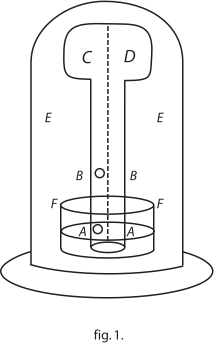
\includegraphics[width=0.4\textwidth]{images/37_3_134r1}\\\textit{[Fig. 2]}
%                        %\caption{Bildbeschreibung}
%                        \end{center}
                    \pstart \textso{Object. 7.} Il reste \`{a} present de rendre raison d'une particularit\'{e} tres considerable \edtext{du phenomene 6}{\lemma{}\Afootnote{du phenomene 6 \textit{ erg.} \textit{ L}}}; puisque sans cela nostre hypothese seroit imparfaite.                         S\c{c}avoir pourquoy une petite bulle estant \edtext{par\"{u}e, au bas}{\lemma{estant}\Afootnote{ \textit{ (1) }\ n\'{e}e au fond \textit{ (2) }\ par\"{u}e, au bas \textit{ L}}} du Matras \textit{A}\edtext{}{\lemma{}\Afootnote{\textit{A}  \textbar\ (il faut voir les figures du \textit{Journal des S\c{c}avans} pag. 134. Juillet 1672, et de la lettre) \textit{ gestr.}\ \textbar\ et \textit{ L}}} et montant jusque \`{a} \textit{B} \edtext{alors la bulle s'etend subitement jusque au haut}{\lemma{\textit{B}}\Afootnote{ \textit{ (1) }\ cet \`{a} dire jusque \`{a} haut \textit{ (2) }\ \textit{B} estant le point \textit{ (3) }\ la liq \textit{ (4) }\ alors [...] haut \textit{ L}}} du Matras\edtext{ \textit{CD} et la liqueur tombe, et remplit jusque \`{a} \textit{F} le vase dans lequel la bouche du Matras trempe. Mais ce qui est remarquable \textit{B} est}{\lemma{Matras}\Afootnote{ \textit{ (1) }\ , et \textit{ (2) }\ \textit{B} estant \textit{ (3) }\ \textit{CD} [...] lequel \textit{(a)}\ le \textit{(b)}\ la bouche [...] est \textit{ L}}} le point, jusque auquel la liqueur\protect\index{Sachverzeichnis}{liqueur}  arrive même apres estre tomb\'{e}e, par la force de l'air qui reste encor dans le Recipient \'{e}puis\'{e} \textit{EE} et qui pousse l'eau outre son niveau \textit{F}. Il semble tres difficile d'en rendre raison, en quelque Hypothese, que la puisse estre, et neantmoins la nostre nous fournit une solution tres ais\'{e}e. Car même pendant que \edtext{le}{\lemma{}\Afootnote{le \textit{ erg.} \textit{ L}}} Matras est plein encor d\'{e}puis \textit{A} jusque en \textit{CD} ou que la liqueur\protect\index{Sachverzeichnis}{liqueur} est 
suspendue, et que la bulle monte entre \textit{A} et \textit{B} l'air du Recipient \textit{EE} soûtient seulement l'eau entre \textit{A} et \textit{B}. Le reste outre \textit{B} et \textit{CD} est soûtenu par la force unitive, car l'eau \textit{AB} se repose immediatement sur le ressort de l'\edtext{air}{\lemma{l'}\Afootnote{ \textit{ (1) }\ eau \textit{ (2) }\ air \textit{ L}}} du Recipient; le reste \textit{B-CD} ne pouuant pas estre soûtenu par l'air, sinon par la mediation de l'eau en \textit{AB}, mais l'eau en \textit{AB}